\documentclass[onecolumn]{article}
\usepackage{graphicx}
\usepackage[utf8]{inputenc} % UTF8 input encoding
\usepackage{microtype} % bedre orddeling & andet typografisk halløj
\usepackage{amsmath, amssymb, mathtools, bm, nicefrac, mathrsfs} % matematik-pakker
\raggedbottom
\newcommand{\sub}[1]{_{\mathrm{#1}}}

\begin{document}
\title{Halfway Project: Exercise 9 - Exponential function (ODE representation)}
\date{}
\author{Mikkel Elkjaer Pedersen}
\maketitle

This short report outlines how the Ordinary Differential Equation (ODE) representaiton of the exponential function may be acchieved.
In short, the object is to calculate $\mathrm{exp}(x)$ for a real number $x$ using the ODE representation of the exponential function given as
\begin{equation}
\frac{dy}{dx} = y, \, y(0) = 1,
\end{equation}
where the latter expression is the initial condition for the exponential function. Knowing the initial condition and the differential equation one
then integrates the differential equation up to the desired real number $x$ to get $\mathrm{exp}(x)$. As with any numerical integration one 
should aim to implement one or more reductions of the argument to avoid integration over too large an interval. For the exponential function the
argument $x$ can be reduced to the interval $[0,1)$ by exploting the following identities:

\begin{equation}
\mathrm{exp}(-x) = \frac{1}{\mathrm{exp}(x)}, \, \mathrm{exp}(x) = \mathrm{exp}\left( \frac{x}{2}\right) ^2.
\label{eqn:reduction}
\end{equation}

Also, for the representation plotted in fig. \ref{fig:exp} the initial condition has been explicitly enforced when performing the integration.
To perform the integration routines from Gnu Scientific Library (GSL) has been used. To utilize the library for solving ODEs the header
\textbf{gsl\_odeiv2.h} must be included in the program. The program should then set up (that is, define) the ODE system. This consists of 
at least a function defining the differential equation and a statement of the dimensionality of the problem. Typically the problem depends
on one or several parameters which should also be comitted to the ODE-system. Additionally, one may include a function to calculate the Jacobian
if this is available for the problem. Once the system is set up the initial conditions of the problem, the initial step size, tolerances and 
the prefered integrator method can be specified to a driver that then automatically combines evolution, stepper and control objects to perform
the integration.
In this project the Runge-Kutta-Fehlberg (4,5) method is chosen as the integrator algorithm as it is a good general-purpose integrator.
The initial guess for a proper step size is $0.1$ while both the relative and absolute tolerances have been set to $1\mathrm{e}-5$. In a main
function the program described above is then called with $x$ being the argument. The range is chosen to be $[-10;10]$ to show that the reductions
work. That is, when the program is called with e.g. $x=7.2$ the program recursively calls itself with $x/=2$ until $x$ is in the desired range
$[0,1)$. The integration is then performed and the result is carried through the levels of recursion where eqn. \ref{eqn:reduction} is then
properly utilized to get the result for $x=7.2$. The result is plotted in fig. \ref{fig:exp} along the exponential function from math.h in GSL.

\begin{figure}
% GNUPLOT: LaTeX picture with Postscript
\begingroup
  \makeatletter
  \providecommand\color[2][]{%
    \GenericError{(gnuplot) \space\space\space\@spaces}{%
      Package color not loaded in conjunction with
      terminal option `colourtext'%
    }{See the gnuplot documentation for explanation.%
    }{Either use 'blacktext' in gnuplot or load the package
      color.sty in LaTeX.}%
    \renewcommand\color[2][]{}%
  }%
  \providecommand\includegraphics[2][]{%
    \GenericError{(gnuplot) \space\space\space\@spaces}{%
      Package graphicx or graphics not loaded%
    }{See the gnuplot documentation for explanation.%
    }{The gnuplot epslatex terminal needs graphicx.sty or graphics.sty.}%
    \renewcommand\includegraphics[2][]{}%
  }%
  \providecommand\rotatebox[2]{#2}%
  \@ifundefined{ifGPcolor}{%
    \newif\ifGPcolor
    \GPcolortrue
  }{}%
  \@ifundefined{ifGPblacktext}{%
    \newif\ifGPblacktext
    \GPblacktexttrue
  }{}%
  % define a \g@addto@macro without @ in the name:
  \let\gplgaddtomacro\g@addto@macro
  % define empty templates for all commands taking text:
  \gdef\gplbacktext{}%
  \gdef\gplfronttext{}%
  \makeatother
  \ifGPblacktext
    % no textcolor at all
    \def\colorrgb#1{}%
    \def\colorgray#1{}%
  \else
    % gray or color?
    \ifGPcolor
      \def\colorrgb#1{\color[rgb]{#1}}%
      \def\colorgray#1{\color[gray]{#1}}%
      \expandafter\def\csname LTw\endcsname{\color{white}}%
      \expandafter\def\csname LTb\endcsname{\color{black}}%
      \expandafter\def\csname LTa\endcsname{\color{black}}%
      \expandafter\def\csname LT0\endcsname{\color[rgb]{1,0,0}}%
      \expandafter\def\csname LT1\endcsname{\color[rgb]{0,1,0}}%
      \expandafter\def\csname LT2\endcsname{\color[rgb]{0,0,1}}%
      \expandafter\def\csname LT3\endcsname{\color[rgb]{1,0,1}}%
      \expandafter\def\csname LT4\endcsname{\color[rgb]{0,1,1}}%
      \expandafter\def\csname LT5\endcsname{\color[rgb]{1,1,0}}%
      \expandafter\def\csname LT6\endcsname{\color[rgb]{0,0,0}}%
      \expandafter\def\csname LT7\endcsname{\color[rgb]{1,0.3,0}}%
      \expandafter\def\csname LT8\endcsname{\color[rgb]{0.5,0.5,0.5}}%
    \else
      % gray
      \def\colorrgb#1{\color{black}}%
      \def\colorgray#1{\color[gray]{#1}}%
      \expandafter\def\csname LTw\endcsname{\color{white}}%
      \expandafter\def\csname LTb\endcsname{\color{black}}%
      \expandafter\def\csname LTa\endcsname{\color{black}}%
      \expandafter\def\csname LT0\endcsname{\color{black}}%
      \expandafter\def\csname LT1\endcsname{\color{black}}%
      \expandafter\def\csname LT2\endcsname{\color{black}}%
      \expandafter\def\csname LT3\endcsname{\color{black}}%
      \expandafter\def\csname LT4\endcsname{\color{black}}%
      \expandafter\def\csname LT5\endcsname{\color{black}}%
      \expandafter\def\csname LT6\endcsname{\color{black}}%
      \expandafter\def\csname LT7\endcsname{\color{black}}%
      \expandafter\def\csname LT8\endcsname{\color{black}}%
    \fi
  \fi
    \setlength{\unitlength}{0.0500bp}%
    \ifx\gptboxheight\undefined%
      \newlength{\gptboxheight}%
      \newlength{\gptboxwidth}%
      \newsavebox{\gptboxtext}%
    \fi%
    \setlength{\fboxrule}{0.5pt}%
    \setlength{\fboxsep}{1pt}%
\begin{picture}(7200.00,4320.00)%
    \gplgaddtomacro\gplbacktext{%
      \csname LTb\endcsname%%
      \put(849,595){\makebox(0,0)[r]{\strut{}$0$}}%
      \csname LTb\endcsname%%
      \put(849,1303){\makebox(0,0)[r]{\strut{}$5000$}}%
      \csname LTb\endcsname%%
      \put(849,2010){\makebox(0,0)[r]{\strut{}$10000$}}%
      \csname LTb\endcsname%%
      \put(849,2718){\makebox(0,0)[r]{\strut{}$15000$}}%
      \csname LTb\endcsname%%
      \put(849,3425){\makebox(0,0)[r]{\strut{}$20000$}}%
      \csname LTb\endcsname%%
      \put(849,4133){\makebox(0,0)[r]{\strut{}$25000$}}%
      \csname LTb\endcsname%%
      \put(951,409){\makebox(0,0){\strut{}$-10$}}%
      \csname LTb\endcsname%%
      \put(2437,409){\makebox(0,0){\strut{}$-5$}}%
      \csname LTb\endcsname%%
      \put(3922,409){\makebox(0,0){\strut{}$0$}}%
      \csname LTb\endcsname%%
      \put(5408,409){\makebox(0,0){\strut{}$5$}}%
      \csname LTb\endcsname%%
      \put(6893,409){\makebox(0,0){\strut{}$10$}}%
    }%
    \gplgaddtomacro\gplfronttext{%
      \csname LTb\endcsname%%
      \put(153,2364){\rotatebox{-270}{\makebox(0,0){\strut{}y}}}%
      \csname LTb\endcsname%%
      \put(3922,130){\makebox(0,0){\strut{}x}}%
      \csname LTb\endcsname%%
      \put(6105,3966){\makebox(0,0)[r]{\strut{}My Exp}}%
      \csname LTb\endcsname%%
      \put(6105,3780){\makebox(0,0)[r]{\strut{}Exp(x) from math.h}}%
    }%
    \gplbacktext
    \put(0,0){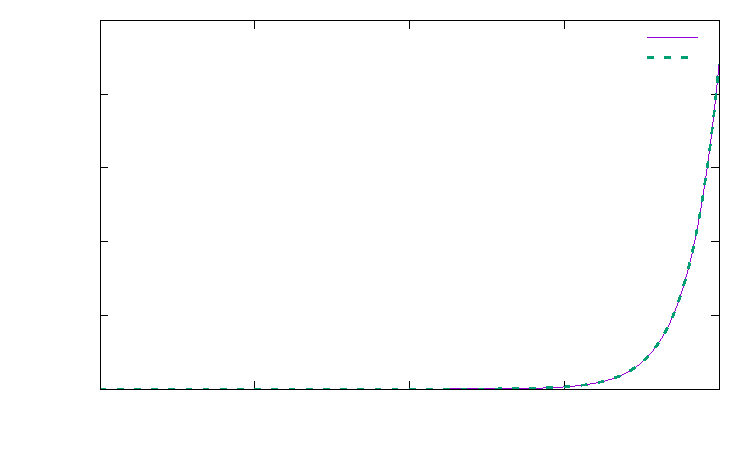
\includegraphics{plot-cairo}}%
    \gplfronttext
  \end{picture}%
\endgroup

	\caption{A plot of the ODE representation of the exponential function and the one from the standard C library math.h in the range
		$[-10,10]$.}
\label{fig:exp}
\end{figure}

\end{document}
